\documentclass[a4paper, 11pt]{article}
\usepackage{comment} % enables the use of multi-line comments (\ifx \fi) 
\usepackage{fullpage} % changes the margin
\usepackage{hyperref}
\usepackage{mathtools}
\usepackage{amsmath}
\usepackage{amssymb}
\usepackage{longtable}
\usepackage{booktabs} % For formal tables
\usepackage[ruled]{algorithm2e} % For algorithms
\renewcommand{\algorithmcfname}{ALGORITHM}
\DeclarePairedDelimiter{\ceil}{\lceil}{\rceil}

\begin{document}

\begin{titlepage}
   \begin{center}
       \vspace*{1cm}
 
       \textbf{\huge{SOEN 6011: SOFTWARE ENGINEERING PROCESSES}}
 
       \vspace{0.5cm}
        \textbf{\huge{Project Deliverable 3}}
 
       \vspace{1.0cm}
       \vskip 1.4in
    
\includegraphics[width=1.0\textwidth]{Concordia.jpg}
       
       \vskip 1.4in
 
       \vspace{0.8cm}
       \textbf{GitHub Repository : \url{https://github.com/Hkohli30/SOEN_6011}}\\
       
        \textbf{Himanshu Kohli}\\
        \textbf{Student Id : 40070839}\\
       Applied Computer Science\\
       Concordia University\\
       
 
   \end{center}
\end{titlepage}

% @author : Himanshu Kohli
% Student ID: 40070839
% Date: 02 August 2019
\noindent
\large\textbf{Problem 5 and 7} \hfill \textbf{Himanshu Kohli} \\
\normalsize SOEN 6011 \hfill \textbf{40070839} \\
Prof. Pankaj Kamthan \hfill Due Date: August 02, 2019 \\


\section{Problem 5: Code Review}
\subsection{Information}

\begin{itemize}
    \item \textbf{Module Name: } B(x,y)
    \item \textbf{Developed By: } Shruthi Kondapura Venkataiah [40091427]
    \item \textbf{Code Review By: } Himanshu Kohli
    \item \textbf{Development End: } July 29,2019
\end{itemize}



\subsection{Introduction}
The relation between the set of input values and the output values is specified as the 'Euler Integral of first kind' more formally known as Beta Function. And the input is set of real values. \newline
The code review is a standard mechanism to avoid Code Smells and to improve the efficiency of the code. The coder used underlining specifications to write code.
\begin{enumerate}
    \item \textbf{Non repeating code:} The code used structures in the code which are non-repeating which enhances readability and faster execution of code
    \item \textbf{Proper commenting } : The coder wrote proper java docs which provided explanation of the function and global variables to understand the code. And avoided obscure commenting.
    \begin{figure}[h]
    \caption{Proper commenting}
    \centering
    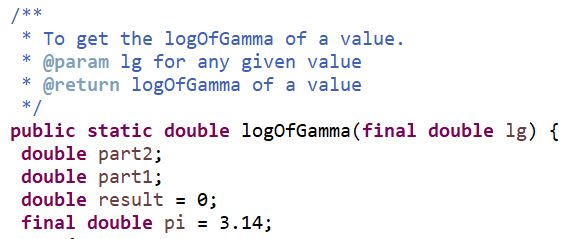
\includegraphics[width=0.40\textwidth]{comment.JPG}
    \end{figure}
    
    \item \textbf{Avoided magic numbers: }The author avoided magic numbers all together in the code which leads to error and reduce efficiency
    \item \textbf{One purpose variable:} Every variable declared has a specific purpose and is not used to hold any other type variables.
    
    \item \textbf{Avoided global variables:} Only one global variable is specified in the program with proper modifiers such as �static� and �final� so as the functions can use the variable. 
    \item \textbf{Good names:} Most of the functions have variables with self-explanatory names which provide enough information for the reader to understand the code. For a function �logOfGamma� the two variables declared are doesn�t have proper naming. 
    \begin{figure}[h]
    \caption{Improper naming}
    \centering
    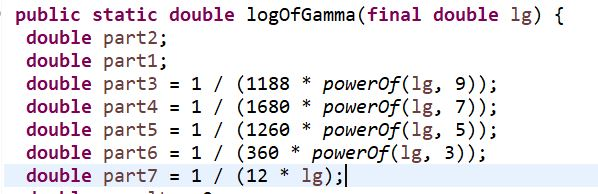
\includegraphics[width=0.40\textwidth]{variableName.JPG}
    \end{figure}
    
    \item \textbf{Proper exception handling:} The coder wrote proper exception handling code which manages the code while run-time execution. \newline 
    \begin{figure}[h]
    \caption{Exception Handling}
    \centering
    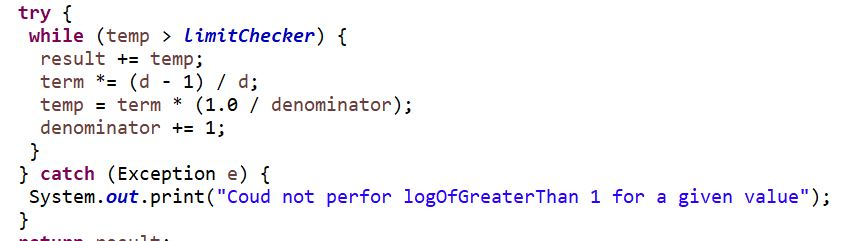
\includegraphics[width=0.49\textwidth]{exception.JPG}
    \end{figure}
    \item \textbf{Methods returning proper results:} All the methods except main method take valid input argument and return the result to be processed and avoid printing statements int them.
    \begin{figure}[h]
    \caption{Methods returning results}
    \centering
    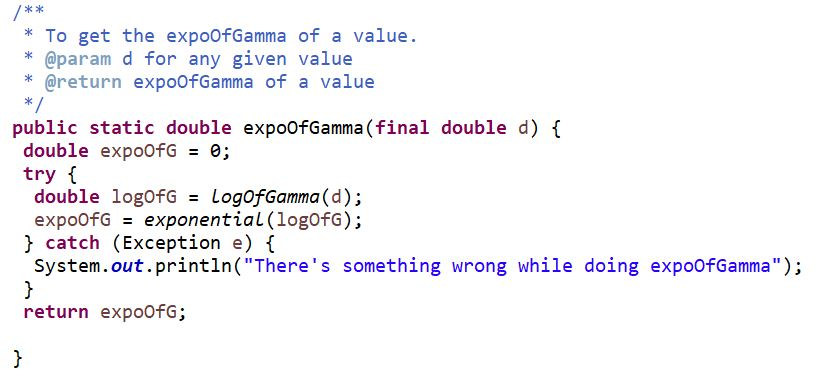
\includegraphics[width=0.49\textwidth]{results.JPG}
    \end{figure}
    
    \item \textbf{Modularity:} Beta Function uses lots of calculations and every function is divided into separate functional modules which makes modification, maintenance and bug detection easier.
\end{enumerate}

\subsection{Coding Standards}
\begin{enumerate}
    \item \textbf{Block statements:} The block statement and the presentation of the curly braces is identical to the pre-decided coding standards
    \item \textbf{Self-descriptive variables:} Some of variable names could have been more descriptive for the reader to understand their proper working.
    \item \textbf{Proper import statements:} The coder use proper import statements while avoiding the �.*� statements.
    \item \textbf{Proper spacing:} Instead of using tab the user has used the 'space bar' which is not according to the pre-decided coding standards.
    
    \item \textbf{Naming convention:} The team pre-decided �camel-casing� methodology for declaring class names, function names and variables which were properly followed in the code.
    \begin{figure}[h]
    \caption{Naming Conventions}
    \centering
    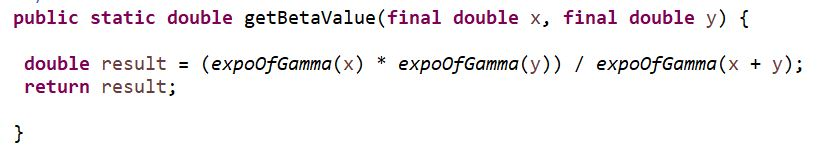
\includegraphics[width=0.49\textwidth]{namingConventions.JPG}
    \end{figure}
    
\end{enumerate}

\section{Problem 7: Function Testing}
\subsection{Introduction}
The function $x^y$ where x and y are variables and the domain is set of real numbers.
\begin{itemize}
    \item \textbf{Module Name: } $x^y$
    \item \textbf{Developed By: } Sanchit Kumar [40081187]
    \item \textbf{https://github.com/san089/SOEN-6011}
    \item \textbf{Code Review By: } Himanshu Kohli
    \item \textbf{Development End: } July 29,2019
\end{itemize}

\subsection{Testing Reports}
\subsubsection{MainTest.java}
All the functions check the input with ($x^y$)
\begin{itemize}

	\item \textbf{Test Case ID: } TC1 \\
	\textbf{Type: } Functional \\
	\textbf{Function Name: }ZeroRaisedToZero\\
	\textbf{Input x,y: } 0,0\\
	\textbf{Expected Result: } 0\\
	\textbf{Original Result: } 0\\
	\textbf{Test Result: } PASS
	
	
	\item \textbf{Test Case ID: } TC2\\
	\textbf{Type: } Functional\\
	\textbf{Function Name: }ZeroRaisedToNegative\\
	\textbf{Input x,y: } 0,-55\\
	\textbf{Expected Result: } 0\\
	\textbf{Original Result: } 0\\
	\textbf{Test Result: } PASS


	\item \textbf{Test Case ID: } TC3\\
	\textbf{Type: } Functional\\
	\textbf{Function Name: }negativeBaseRootError\\
	\textbf{Input x,y: } -2,-1.99\\
	\textbf{Expected Result: } NOTHING\\
	\textbf{Original Result: } NOTHING\\
	\textbf{Test Result: } PASS
	
	
	\item \textbf{Test Case ID: } TC4\\
	\textbf{Type: } Functional\\
	\textbf{Function Name: }notANumberInput\\
	\textbf{Input x,y: } xyz\\
	\textbf{Expected Result: } Exception [invalid input]\\
	\textbf{Original Result: } Exception [invalid input]\\
	\textbf{Test Result: } PASS

\end{itemize}

\subsubsection{pow.java}

\begin{itemize}
	\item \textbf{Test Case ID: } TC5\\
	\textbf{Type: } Functional\\
	\textbf{Function Name: } getSignToMultiply\\
	\textbf{Input x,y: } 100,5\\
	\textbf{Expected Result: } 1E10\\
	\textbf{Original Result: } 1E10\\
	\textbf{Test Result: } PASS
	
	\item \textbf{Test Case ID: } TC6\\
	\textbf{Type: } Functional\\
	\textbf{Function Name: }getPowResult \\
	\textbf{Input x,y: } 100,5\\
	\textbf{Expected Result: } 1E10\\
	\textbf{Original Result: } 1E10\\
	\textbf{Test Result: } PASS
	
	\item \textbf{Test Case ID: } TC7\\
	\textbf{Type: } Functional\\
	\textbf{Function Name: } getPowResultTimeTest\\
	\textbf{Input x,y: } 311,5\\
	\textbf{Expected Result: } 1E10\\
	\textbf{Original Result: } 1E10\\
	\textbf{Test Result: } PASS
	
	\item \textbf{Test Case ID: } TC8\\
	\textbf{Type: } Functional\\
	\textbf{Function Name: } getExponent\\
	\textbf{Input x,y: } 16666666666,20\\
	\textbf{Expected Result: } 2.73511123E204\\
	\textbf{Original Result: } 2.73511123E204\\
	\textbf{Test Result: } PASS
	
	\item \textbf{Test Case ID: } TC9\\
	\textbf{Type: } Functional\\
	\textbf{Function Name: }getLn \\
	\textbf{Input x: } 2150\\
	\textbf{Expected Result: } 4.07347147E74\\
	\textbf{Original Result: } 4.07347147E74\\
	\textbf{Test Result: } PASS
	
	\item \textbf{Test Case ID: } TC10\\
	\textbf{Type: } Functional\\
	\textbf{Function Name: }getSmallerValue \\   
	\textbf{Input number,pointValue } 1236826381683681263868162836,28\\
	\textbf{Expected Result: } 0.1236826381683681263868162836\\
	\textbf{Original Result: } 0.1236826381683681263868162836\\
	\textbf{Test Result: } PASS
	
	\item \textbf{Test Case ID: } TC11\\
	\textbf{Type: } Functional\\
	\textbf{Function Name: } numSignificantDigits\\
	\textbf{Input number} 10000.00000\\
	\textbf{Expected Result: } 5\\
	\textbf{Original Result: } 5\\
	\textbf{Test Result: } PASS
	
	
	\item \textbf{Test Case ID: } TC12\\
	\textbf{Type: } Functional\\
	\textbf{Function Name: } getXValForLog\\
	\textbf{Input number } -0.8181818182\\
	\textbf{Expected Result: } 0.1\\
	\textbf{Original Result: } 0.1\\
	\textbf{Test Result: } PASS\\
	
	
	\item \textbf{Test Case ID: } TC13\\
	\textbf{Type: } Functional\\
	\textbf{Function Name: } getPower\\
	\textbf{Input x,y } 2.42,2\\
	\textbf{Expected Result: } 5.8564\\
	\textbf{Original Result: } 5.8564\\
	\textbf{Test Result: } PASS\\
	
\end{itemize}

\subsubsection{Summary Table}

\begin{center}
\begin{longtable}{|l|l|l|}
\caption{Test case summary table.} 
\label{tab:long} \\

\hline \multicolumn{1}{|c|}{\textbf{Test Case ID#}} & \multicolumn{1}{c|}{\textbf{Test Case Status}}\\ \hline 
\endfirsthead

\multicolumn{2}{c}%
{{\bfseries \tablename\ \thetable{} -- continued from previous page}} \\
\hline \multicolumn{1}{|c|}{\textbf{Test Case ID}} & \multicolumn{1}{c|}{\textbf{Test Case Status}}  \\ \hline 
\endhead

\hline \multicolumn{2}{|r|}{{Continued on next page}} \\ \hline
\endfoot

\hline \hline
\endlastfoot

TC1 & PASS\\
TC2 & PASS \\
TC3 & PASS\\
TC4 & PASS\\
TC5 & PASS\\
TC6 & PASS\\
TC7 & PASS\\
TC8 & PASS\\
TC9 & PASS\\
TC10 & PASS\\
TC11 & PASS\\
TC12 & PASS \\
\end{longtable}
\end{center}

\subsubsection{Remarks}

\begin{enumerate}
    \item For all the test cases there were no JavaDocs writeen by the coder.
    \item For functions of TC1 and TC2 there is voilation of coding standards.
    \item There is use of BigDecimal variables and BigDecimal library in the coding.
    \item The results are highly accurate with the calculator results.
\end{enumerate}

\begin{thebibliography}{}
\bibitem{ref} 
Robert L. Glass: Facts and Fallacies of Software Engineering; Addison Wesley, 2003. ISBN-13: 978-0321117427.
\bibitem{oracle}
Oracle Corporation. Code Conventions for the Java Programming Language.
\url{http://www.oracle.com/technetwork/java/codeconvtoc-136057.html}
\bibitem{google} Google Inc. Google Java Style. \url{https://google.github.io/styleguide/javaguide.html}
\bibitem{app}Peter Grogono. Course notes for COMP6441: Advanced Programming Practices. Concordia University, 2007.  
\bibitem{mit} Reading 4: Code  \url{http://web.mit.edu/6.005/www/fa15/classes/04-code-review/}

\bibitem{vogella}
Unit Testing with JUnit - Tutorial
\url{https://www.vogella.com/tutorials/JUnit/article.html}
\end{thebibliography}

\end{document}